\section{Implementation}

We have written a prototype compiler for \sysname that is implemented in roughly 5500 lines of F\# code. The compiler includes command-line flags for enabling or disabling the use of the BGP MED attribute, AS path prepending, the commonly used no-export community, as well as for ensuring at least k-failure safety for user-sepcified aggregates. Users see only ever see the high-level constraint-based language presented in Section~\ref{sec:motivation}.

\para{PG construction}

Constructing automata for extended regular expressions (regular expressions including negation and intersection) are known to have high complexity~\ref{bib:todo}. Our \sysname compiler uses regular expressions derivatives~\ref{bib:todo} with character classes to construct deterministic automata for extended regular expressions over large alphabets efficiently. Since regular expressions are defined over a finite alphabet, and since much of the AS topology is unknown, we set the alphabet to include all uniquely referenced external ASes in the policy. Similarly, to model the unknown external AS topology beyond immediate peers, we include a special topology node to represent any unknown location.

Rather than construct the product graph in full, our implementation prevents exploring parts of the graph when no accepting state is reachable in any of the corresponding regular automata during construction.

\para{PG Minimization}

Our compiler uses a fast algorithm for computing graph dominators by storing sets of dominators in a compact representation known as a dominator tree~\ref{bib:todo}. 


When computing local preferences and failure safety, as described in Section~\ref{sec:compilation}, the compiler performs memoization of the ``can prefer'' relation. \todo{this needs work}

We have evaluated our compiler by translating and compiling real-world network configurations for data centers and a core backbone network into \sysname. We evaluate our compiler by measuring compilation times for these policies across topologies of different sizes.

\begin{figure}[t!]
\centering
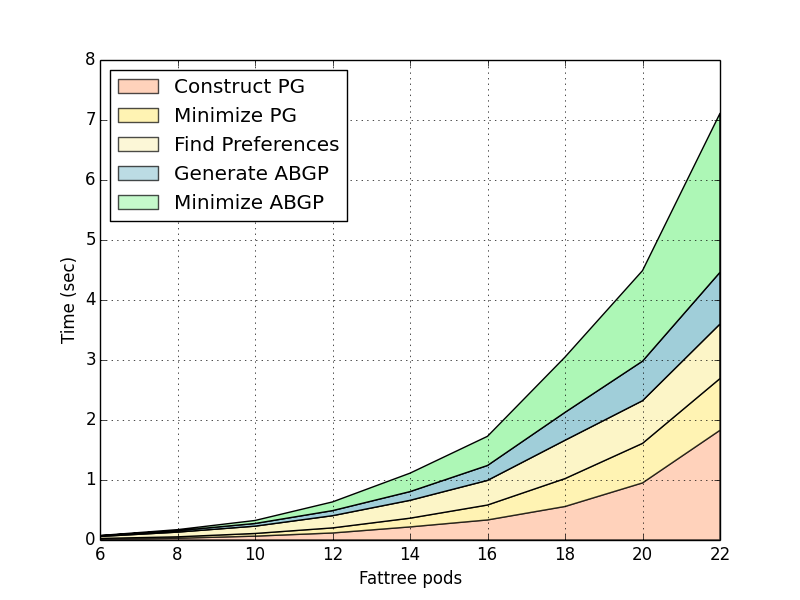
\includegraphics[width=\columnwidth]{figures/compilation-times-dc.png}
\label{fig:compilation-times-dc}
\caption{Data center compilation times.}
\end{figure}

\begin{figure}[t!]
\centering
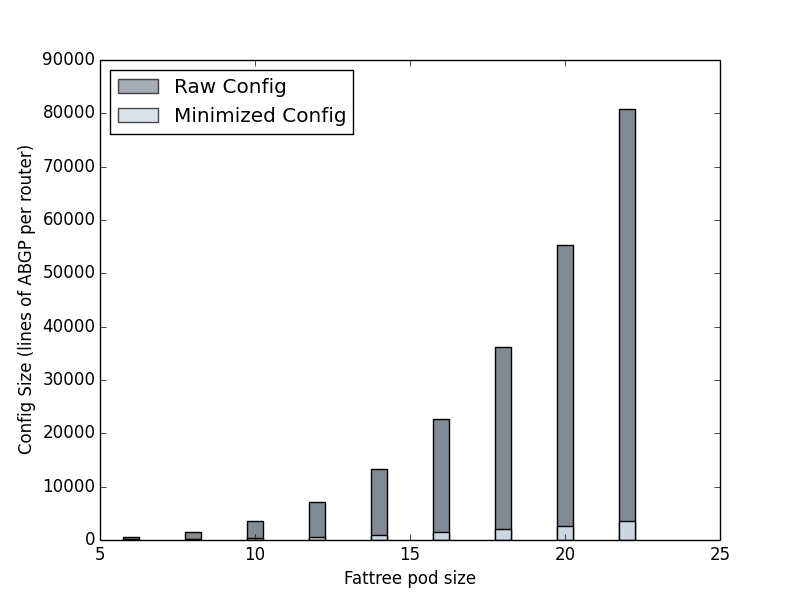
\includegraphics[width=\columnwidth]{figures/config-compression-dc.png}
\label{fig:compilation-compression-dc}
\caption{Data center config minimization.}
\end{figure}